
%{{第四十回}}{第四十回}}

\chapter{史太君两宴大观园 金鸳鸯三宣牙牌令}\label{part0044_split_000.htmlux5cux23calibre_pb_0}

{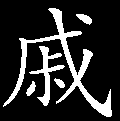
\includegraphics[width=3mm]{../Images/00005}两宴不觉已深秋,惜春只如画春游。可怜富贵谁能保,只有恩情得到头。}

话说宝玉听了,忙进来看时,只见琥珀站在屏风跟前说:``快去吧,立等你说话呢。''宝玉来至上房,只见贾母正和王夫人、众姊妹商议给史湘云还席。宝玉因说道:``我有个主意。既没有外客,吃的东西也别定了样数,谁素日爱吃的拣样儿做几样。也不要按桌席,每人跟前摆一张高几,各人爱吃的东西一两样,再一个什锦攒心盒子,自斟壶,岂不别致。''贾母听了,说``很是'',忙命传与厨房:``明日就拣我们爱吃的东西作了,按着人数,再装了盒子来。早饭也摆在园里吃。''商议之间早又掌灯,一夕无话。

次日清早起来,可喜这日天气清朗。李纨侵晨先起,看着老婆子丫头们扫那些落叶,{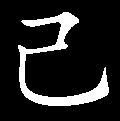
\includegraphics[width=3mm]{../Images/00003}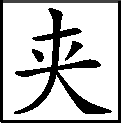
\includegraphics[width=3mm]{../Images/00012}\footnotesize \kaishu 是八月尽。}并擦抹桌椅,预备茶酒器皿。只见丰儿带了刘姥姥板儿进来,说``大奶奶倒忙的紧。''李纨笑道:``我说你昨儿去不成,只忙着要去。''刘姥姥笑道:``老太太留下我,叫我也热闹一天去。''丰儿拿了几把大小钥匙,说道:``我们奶奶说了,外头的高几恐不够使,不如开了楼把那收着的拿下来使一天罢。奶奶原该亲自来的,因和太太说话呢,请大奶奶开了,带着人搬罢。''李氏便令素云接了钥匙,又令婆子出去把二门上的小厮叫几个来。李氏站在大观楼下往上看,令人上去开了缀锦阁,一张一张往下抬。小厮、老婆子、丫头一齐动手,抬了二十多张下来。李纨道:``好生着,别慌慌张张鬼赶来似的,仔细碰了牙子。''又回头向刘姥姥笑道:``姥姥,你也上去瞧瞧。''刘姥姥听说,巴不得一声儿,便拉了板儿登梯上去进里面,只见乌压压的堆着些围屏、桌椅、大小花灯之类,虽不大认得,只见五彩炫耀,各有奇妙。念了几声佛,便下来了。然后锁上门,一齐才下来。李纨道:``恐怕老太太高兴,越性把舡上划子、篙桨、遮阳幔子都搬了下来预备着。''众人答应,复又开了,色色的搬了下来。令小厮传驾娘们到舡坞里撑出两只船来。

正乱着安排,只见贾母已带了一群人进来了。李纨忙迎上去,笑道:``老太太高兴,倒进来了。我只当还没梳头呢,才撷了菊花要送去。''一面说,一面碧月早捧过一个大荷叶式的翡翠盘子来,里面盛着各色的折枝菊花。贾母便拣了一朵大红的簪了鬓上。因回头看见了刘姥姥,忙笑道:``过来带花儿。''一语未完,凤姐便拉过刘姥姥,笑道:``让我打扮你。''说着,将一盘子花横三竖四的插了一头。贾母和众人笑的了不得。刘姥姥笑道:``我这头也不知修了什么福,今儿这样体面起来。''众人笑道:``你还不拔下来摔到他脸上呢,把你打扮的成了个老妖精了。''刘姥姥笑道:``我虽老了,年轻时也风流,爱个花儿粉儿的,今儿老风流才好。''

说笑之间,已来至沁芳亭子上。丫鬟们抱了一个大锦褥子来,铺在栏杆榻板上。贾母倚柱坐下,命刘姥姥也坐在旁边,因问他:``这园子好不好?''刘姥姥念佛说道:``我们乡下人到了年下,都上城来买画儿贴。时常闲了,大家都说,怎么得也到画儿上去逛逛。想着那个画儿也不过是假的,那里有这个真地方呢。谁知我今儿进这园里一瞧,竟比那画儿还强十倍。怎么得有人也照着这个园子画一张,我带了家去,给他们见见,死了也得好处。''贾母听说,便指着惜春笑道:``你瞧我这个小孙女儿,他就会画。等明儿叫他画一张如何?''刘姥姥听了,喜的忙跑过来,拉着惜春说道:``我的姑娘,你这么大年纪儿,又这么个好模样,还有这个能干,别是神仙托生的罢。''

贾母少歇一回,自然领着刘姥姥都见识见识。先到了潇湘馆。一进门,只见两边翠竹夹路,土地下苍苔布满,中间羊肠一条石子漫的路。刘姥姥让出路来与贾母众人走,自己却赾走土地。琥珀拉着他说道:``姥姥,你上来走,仔细苍苔滑了。''刘姥姥道:``不相干的,我们走熟了的,姑娘们只管走罢。可惜你们的那绣鞋,别沾脏了。''他只顾上头和人说话,不防底下果踩滑了,咕咚一跤跌倒。众人拍手都哈哈的笑起来。贾母笑骂道:``小蹄子们,还不搀起来,只站着笑。''说话时,刘姥姥已爬了起来,自己也笑了,说道:``才说嘴就打了嘴。''贾母问他:``可扭了腰了不曾?叫丫头们捶一捶。''刘姥姥道:``那里说的我这么娇嫩了。那一天不跌两下子,都要捶起来,还了得呢。''

紫鹃早打起湘帘,贾母等进来坐下。林黛玉亲自用小茶盘捧了一盖碗茶来奉与贾母。王夫人道:``我们不吃茶,姑娘不用倒了。''林黛玉听说,便命丫头把自己窗下常坐的一张椅子挪到下首,请王夫人坐了。刘姥姥因见窗下案上设着笔砚,又见书架上磊着满满的书,刘姥姥道:``这必定是那位哥儿的书房了。''贾母笑指黛玉道:``这是我这外孙女儿的屋子。''刘姥姥留神打量了黛玉一番,方笑道:``这那像个小姐的绣房,竟比那上等的书房还好。''贾母因问:``宝玉怎么不见?''众丫头们答说:``在池子里舡上呢。''贾母道:``谁又预备下舡了?''李纨忙回说:``才开楼拿几,我恐怕老太太高兴,就预备下了。''贾母听了方欲说话时,有人回说:``姨太太来了。''贾母等刚站起来,只见薛姨妈早进来了,一面归坐,笑道:``今儿老太太高兴,这早晚就来了。''贾母笑道:``我才说来迟了的要罚他,不想姨太太就来迟了。''

说笑一会,贾母因见窗上纱的颜色旧了,便和王夫人说道:``这个纱新糊上好看,过了后来就不翠了。这个院子里头又没有个桃杏树,这竹子已是绿的,再拿这绿纱糊上反不配。我记得咱们先有四五样颜色糊窗的纱呢,明儿给他把这窗上的换了。''凤姐儿忙道:``昨儿我开库房,看见大板箱里还有好些匹银红蝉翼纱,也有各样折枝花样的,也有流云万福花样的,也有百蝶穿花花样的,颜色又鲜,纱又轻软,我竟没见过这样的。拿了两匹出来,作两床绵纱被,想来一定是好的。''贾母听了笑道:``呸,人人都说你没有不经过不见过,连这个纱还不认得呢,明儿还说嘴。''薛姨妈等都笑说:``凭他怎么经过见过,如何敢比老太太呢。老太太何不教导了他,我们也听听。''凤姐儿也笑说:``好祖宗,教给我罢。''

贾母笑向薛姨妈众人道:``那个纱,比你们的年纪还大呢。怪不得他认作蝉翼纱,原也有些像,不知道的,都认作蝉翼纱。正经名字叫作`软烟罗'。''凤姐儿道:``这个名儿也好听。只是我这么大了,纱罗也见过几百样,从没听见过这个名色。''贾母笑道:``你能够活了多大,见过几样没处放的东西,就说嘴来了。那个软烟罗只有四样颜色:一样雨过天晴,一样秋香色,一样松绿的,一样就是银红的。若是做了帐子,糊了窗屉,远远的看着,就似烟雾一样,所以叫作`软烟罗',那银红的又叫作`霞影纱'。如今上用的府纱也没有这样软厚轻密的了。''

薛姨妈笑道:``别说凤丫头没见,连我也没听见过。''凤姐儿一面说,早命人取了一匹来了。贾母说:``可不是这个!先时原不过是糊窗屉,后来我们拿这个作被作帐子,试试也竟好。明儿就找出几匹来,拿银红的替他糊窗子。''凤姐答应着。众人都看了,称赞不已。刘姥姥也觑着眼看个不了,念佛说道:``我们想他作衣裳也不能,拿着糊窗子,岂不可惜?''贾母道:``倒是做衣裳不好看。''凤姐忙把自己身上穿的一件大红绵纱袄子襟儿拉了出来,向贾母薛姨妈道:``看我的这袄儿。''贾母薛姨妈都说:``这也是上好的了,这是如今的上用内造的,竟比不上这个。''凤姐儿道:``这个薄片子,还说是上用内造呢,竟连官用的也比不上了。''贾母道:``再找一找,只怕还有青的。若有时都拿出来,送这刘亲家两匹,做一个帐子我挂,下剩的添上里子,做些夹背心子给丫头们穿,白收着霉坏了。''凤姐忙答应了,仍令人送去。

贾母起身笑道:``这屋里窄,再往别处逛去。''刘姥姥念佛道:``人人都说大家子住大房。昨儿见了老太太正房,配上大箱大柜大桌子大床,果然威武。那柜子比我们那一间房子还大还高。怪道后院子里有个梯子。我想并不上房晒东西,预备个梯子作什么?后来我想起来,定是为开顶柜收放东西,非离了那梯子,怎么得上去呢。如今又见了这小屋子,更比大的越发齐整了。满屋里的东西都只好看,都不知叫什么,我越看越舍不得离了这里。''凤姐道:``还有好的呢,我都带你去瞧瞧。''

说着,一径离了潇湘馆,远远望见池中一群人在那里撑舡。贾母道:``他们既预备下船,咱们就坐。''一面说着,便向紫菱洲、蓼溆一带走来。未至池前,只见几个婆子手里都捧着一色捏丝戗金五彩大盒子走来。凤姐忙问王夫人早饭在那里摆。王夫人道:``问老太太在那里,就在那里罢了。''贾母听说,便回头说:``你三妹妹那里就好。你就带了人摆去,我们从这里坐了舡去。''

凤姐听说,便回身同了探春、李纨、鸳鸯、琥珀带着端饭的人等,抄着近路到了秋爽斋,就在晓翠堂上调开桌案。鸳鸯笑道:``天天咱们说外头老爷们吃酒吃饭都有一个篾片相公,拿他取笑儿。咱们今儿也得了一个女篾片了。''李纨是个厚道人,听了不解。凤姐儿却知是说的是刘姥姥了,也笑说道:``咱们今儿就拿他取个笑儿。''二人便如此这般的商议。李纨笑劝道:``你们一点好事也不做,又不是个小孩儿,还这么淘气,仔细老太太说。''鸳鸯笑道:``很不与你相干,有我呢。''

正说着,只见贾母等来了,各自随便坐下。先着丫鬟端过两盘茶来,大家吃毕。凤姐手里拿着西洋布手巾,裹着一把乌木三镶银箸,敁敠人位,按席摆下。贾母因说:``把那一张小楠木桌子抬过来,让刘亲家近我这边坐着。''众人听说,忙抬了过来。凤姐一面递眼色与鸳鸯,鸳鸯便拉了刘姥姥出去,悄悄的嘱咐了刘姥姥一席话,又说:``这是我们家的规矩,若错了我们就笑话呢。''调停已毕,然后归坐。薛姨妈是吃过饭来的,不吃,只坐在一边吃茶。{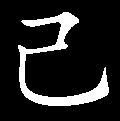
\includegraphics[width=3mm]{../Images/00003}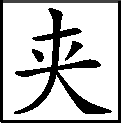
\includegraphics[width=3mm]{../Images/00012}\footnotesize \kaishu 妙!若只管写薛姨妈来则吃饭,则成何文理?}贾母带着宝玉、湘云、黛玉、宝钗一桌,王夫人带着迎春姊妹三个人一桌,刘姥姥傍着贾母一桌。贾母素日吃饭,皆有小丫鬟在旁边,拿着漱盂、麈尾、巾帕之物。如今鸳鸯是不当这差的了,今日鸳鸯偏接过麈尾来拂着。丫鬟们知道他要撮弄刘姥姥,便躲开让他。鸳鸯一面侍立,一面悄向刘姥姥说道:``别忘了。''刘姥姥道:``姑娘放心。''那刘姥姥入了坐,拿起箸来,沉甸甸的不伏手。原是凤姐和鸳鸯商议定了,单拿一双老年四楞象牙镶金的筷子与刘姥姥。刘姥姥见了,说道:``这叉爬子比俺那里铁锨还沉,那里犟的过他。''说的众人都笑起来。

只见一个媳妇端了一个盒子站在当地,一个丫鬟上来揭去盒盖,里面盛着两碗菜。李纨端了一碗放在贾母桌上。凤姐儿偏拣了一碗鸽子蛋放在刘姥姥桌上。贾母这边说声``请'',刘姥姥便站起身来,高声说道:``老刘,老刘,食量大似牛,吃一个老母猪不抬头。''自己却鼓着腮不语。

众人先是发怔,后来一听,上上下下都哈哈的大笑起来。史湘云撑不住,一口饭都喷了出来;林黛玉笑岔了气,伏着桌子``嗳哟'';宝玉早滚到贾母怀里,贾母笑的搂着宝玉叫``心肝'';王夫人笑的用手指着凤姐儿,只说不出话来;薛姨妈也撑不住,口里茶喷了探春一裙子;探春手里的饭碗都合在迎春身上;惜春离了坐位,拉着他奶母叫揉一揉肠子。地下的无一个不弯腰屈背,也有躲出去蹲着笑去的,也有忍着笑上来替他姊妹换衣裳的,独有凤姐鸳鸯二人撑着,还只管让刘姥姥。

刘姥姥拿起箸来,只觉不听使,又说道:``这里的鸡儿也俊,下的这蛋也小巧,怪俊的。我且肏攮一个。''众人方住了笑,听见这话又笑起来。贾母笑的眼泪出来,琥珀在后捶着。贾母笑道:``这定是凤丫头促狭鬼儿闹的,快别信他的话了。''那刘姥姥正夸鸡蛋小巧,要肏攮一个,凤姐儿笑道:``一两银子一个呢,你快尝尝罢,那冷了就不好吃了。''刘姥姥便伸箸子要夹,那里夹的起来,满碗里闹了一阵,好容易撮起一个来,才伸着脖子要吃,偏又滑下来滚在地下,忙放下箸子要亲自去捡,早有地下的人捡了出去了。刘姥姥叹道:``一两银子,也没听见响声儿就没了。''众人已没心吃饭,都看着他笑。

贾母又说:``这会子又把那个筷子拿了出来,又不请客摆大筵席。都是凤丫头支使的,还不换了呢。''地下的人原不曾预备这牙箸,本是凤姐和鸳鸯拿了来的,听如此说,忙收了过去,也照样换上一双乌木镶银的。刘姥姥道:``去了金的,又是银的,到底不及俺们那个伏手。''凤姐儿道:``菜里若有毒,这银子下去了就试的出来。''刘姥姥道:``这个菜里若有毒,俺们那菜都成了砒霜了。那怕毒死了也要吃尽了。''贾母见他如此有趣,吃的又香甜,把自己的也都端过来与他吃。又命一个老嬷嬷来,将各样的菜给板儿夹在碗上。

一时吃毕,贾母等都往探春卧室中去说闲话。这里收拾过残桌,又放了一桌。刘姥姥看着李纨与凤姐儿对坐着吃饭,叹道:``别的罢了,我只爱你们家这行事。怪道说`礼出大家'。''凤姐儿忙笑道:``你可别多心,才刚不过大家取笑儿。''一言未了,鸳鸯也进来笑道:``姥姥别恼,我给你老人家赔个不是。''刘姥姥笑道:``姑娘说那里话,咱们哄着老太太开个心儿,可有什么恼的!你先嘱咐我,我就明白了,不过大家取个笑儿。我要心里恼,也就不说了。''鸳鸯便骂人``为什么不倒茶给姥姥吃?''刘姥姥忙道:``刚才那个嫂子倒了茶来,我吃过了。姑娘也该用饭了。''凤姐儿便拉鸳鸯:``你坐下和我们吃了罢,省的回来又闹。''鸳鸯便坐下了。婆子们添上碗箸来,三人吃毕。

刘姥姥笑道:``我看你们这些人都只吃这一点儿就完了,亏你们也不饿。怪只道风儿都吹的倒。''鸳鸯便问:``今儿剩的菜不少,都那去了?''婆子们道:``都还没散呢,在这里等着一齐散与他们吃。''鸳鸯道:``他们吃不了这些,挑两碗给二奶奶屋里平丫头送去。''凤姐儿道:``他早吃了饭了,不用给他。''鸳鸯道:``他不吃了,喂你们的猫。''婆子听了,忙拣了两样拿盒子送去。鸳鸯道:``素云那去了?''李纨道:``他们都在这里一处吃,又找他作什么。''鸳鸯道:``这就罢了。''凤姐儿道:``袭人不在这里,你倒是叫人送两样给他去。''鸳鸯听说,便命人也送两样去后,鸳鸯又问婆子们:``回来吃酒的攒盒可装上了?''婆子道:``想必还得一会子。''鸳鸯道:``催着些儿。''婆子应喏了。

凤姐儿等来至探春房中,只见他娘儿们正说笑。探春素喜阔朗,这三间屋子并不曾隔断。当地放着一张花梨大理石大案,案上磊着各种名人法帖,并数十方宝砚,各色笔筒,笔海内插的笔如树林一般。那一边设着斗大的一个汝窑花囊,插着满满的一囊水晶球儿的白菊。西墙上当中挂着一大幅米襄阳《烟雨图》,左右挂着一副对联,乃是颜鲁公墨迹,其词云:

烟霞闲骨格,泉石野生涯。

案上设着大鼎。左边紫檀架上放着一个大观窑的大盘,盘内盛着数十个娇黄玲珑大佛手。右边洋漆架上悬着一个白玉比目磬,旁边挂着小锤。

那板儿略熟了些,便要摘那锤子要击,丫鬟们忙拦住他。他又要那佛手吃,探春拣了一个与他说:``顽罢,吃不得的。''东边便设着卧榻,拔步床上悬着葱绿双绣花卉草虫的纱帐。板儿又跑过来看,说:``这是蝈蝈,这是蚂蚱。''刘姥姥忙打了他一巴掌,骂道:``下作黄子,没干没净的乱闹。倒叫你进来瞧瞧,就上脸了。''打的板儿哭起来,众人忙劝解方罢。

贾母因隔着纱窗往后院内看了一回,说道:``后廊檐下的梧桐也好了,就只细些。''正说话,忽一阵风过,隐隐听得鼓乐之声。贾母问``是谁家娶亲呢?这里临街倒近。''王夫人等笑回道:``街上的那里听的见,这是咱们的那十几个女孩子们演习吹打呢。''贾母便笑道:``既是他们演,何不叫他们进来演习。他们也逛一逛,咱们可又乐了。''凤姐听说,忙命人出去叫来,又一面吩咐摆下条桌,铺上红毡子。

贾母道:``就铺排在藕香榭的水亭子上,借着水音更好听。回来咱们就在缀锦阁底下吃酒,又宽阔,又听的近。''众人都说那里好。贾母向薛姨妈笑道:``咱们走罢。他们姊妹们都不大喜欢人来坐着,怕脏了屋子。咱们别没眼色,正经坐一回子船喝酒去。''说着大家起身便走。探春笑道:``这是那里的话,求着老太太姨太太来坐坐还不能呢。''贾母笑道:``我的这三丫头却好,只有两个玉儿可恶。回来吃醉了,咱们偏往他们屋里闹去。''

说着,众人都笑了,一齐出来。走不多远,已到了荇叶渚。那姑苏选来的几个驾娘早把两只棠木舫撑来,众人扶了贾母、王夫人、薛姨妈、刘姥姥、鸳鸯、玉钏儿上了这一只,落后李纨也跟上去。凤姐儿也上去,立在舡头上,也要撑舡。贾母在舱内道:``这不是顽的,虽不是河里,也有好深的。你快不给我进来。''凤姐儿笑道:``怕什么!老祖宗只管放心。''说着便一篙点开。到了池当中,舡小人多,凤姐只觉乱晃,忙把篙子递与驾娘,方蹲下了。然后迎春姊妹等并宝玉上了那只,随后跟来。其馀老嬷嬷、散众丫鬟俱沿河随行。宝玉道:``这些破荷叶可恨,怎么还不叫人来拔去。''宝钗笑道:``今年这几日,何曾饶了这园子闲了,天天逛,那里还有叫人来收拾的工夫。''林黛玉道:``我最不喜欢李义山的诗,只喜他这一句`留得残荷听雨声'\href{../Text/part0044_split_000.html\#lnkback_1_a}{\textsuperscript{①}}。偏你们又不留着残荷了。''宝玉道:``果然好句,以后咱们就别叫人拔去了。''说着已到了花溆的萝港之下,觉得阴森透骨,两滩上衰草残菱,更助秋情。

贾母因见岸上的清厦旷朗,便问``这是你薛姑娘的屋子不是?''众人道:``是。''贾母忙命拢岸,顺着云步石梯上去,一同进了蘅芜苑,只觉异香扑鼻。那些奇草仙藤愈冷愈苍翠,都结了实,似珊瑚豆子一般,累垂可爱。及进了房屋,雪洞一般,一色玩器全无,案上只有一个土定瓶中供着数枝菊花,并两部书,茶奁茶杯而已。床上只吊着青纱帐幔,衾褥也十分朴素。

贾母叹道:``这孩子太老实了。你没有陈设,何妨和你姨娘要些。我也不理论,也没想到,你们的东西自然在家里没带了来。''说着,命鸳鸯去取些古董来,又嗔着凤姐儿:``不送些玩器来与你妹妹,这样小器。''王夫人凤姐儿等都笑回说:``他自己不要的。我们原送了来,他都退回去了。''薛姨妈也笑说:``他在家里也不大弄这些东西的。''贾母摇头道:``使不得。虽然他省事,倘或来一个亲戚,看着不像;二则年轻的姑娘们,房里这样素净,也忌讳。我们这老婆子,越发该住马圈去了。你们听那些书上戏上说的小姐们的绣房,精致的还了得呢。他们姊妹们虽不敢比那些小姐们,也不要很离了格儿。有现成的东西,为什么不摆?若很爱素净,少几样倒使得。我最会收拾屋子的,如今老了,没有这些闲心了。他们姊妹们也还学着收拾的好,只怕俗气,有好东西也摆坏了。我看他们还不俗。如今让我替你收拾,包管又大方又素净。我的梯己两件,收到如今,没给宝玉看见过,若经了他的眼,也没了。''说着叫过鸳鸯来,亲吩咐道:``你把那石头盆景儿和那架纱桌屏,还有个墨烟冻石鼎,这三样摆在这案上就够了。再把那水墨字画白绫帐子拿来,把这帐子也换了。''鸳鸯答应着,笑道:``这些东西都搁在东楼上的不知那个箱子里,还得慢慢找去,明儿再拿去也罢了。''贾母道:``明日后日都使得,只别忘了。''说着,坐了一回方出来,一径来至缀锦阁下。文官等上来请过安,因问``演习何曲''。贾母道:``只拣你们生的演习几套罢。''文官等下来,往藕香榭去不提。

这里凤姐儿已带着人摆设整齐,上面左右两张榻,榻上都铺着锦裀蓉簟,每一榻前有两张雕漆几,也有海棠式的,也有梅花式的,也有荷叶式的,也有葵花式的,也有方的,也有圆的,其式不一。一个上面放着炉瓶,一分攒盒,一个上面空设着,预备放人所喜食物。上面二榻四几,是贾母薛姨妈;下面一椅两几,是王夫人的,馀者都是一椅一几。东边是刘姥姥,刘姥姥之下便是王夫人。西边便是史湘云,第二便是宝钗,第三便是黛玉,第四迎春、探春、惜春挨次下去,宝玉在末。李纨凤姐二人之几设于三层槛内,二层纱厨之外。攒盒式样,亦随几之式样。每人一把乌银洋錾自斟壶,一个十锦珐琅杯。

大家坐定,贾母先笑道:``咱们先吃两杯,今日也行一令才有意思。''薛姨妈等笑道:``老太太自然有好酒令,我们如何会呢,安心要我们醉了。我们都多吃两杯就有了。''贾母笑道:``姨太太今儿也过谦起来,想是厌我老了。''薛姨妈笑道:``不是谦,只怕行不上来倒是笑话了。''王夫人忙笑道:``便说不上来,就便多吃一杯酒,醉了睡觉去,还有谁笑话咱们不成。''薛姨妈点头笑道:``依令。老太太到底吃一杯令酒才是。''贾母笑道:``这个自然。''说着便吃了一杯。

凤姐儿忙走至当地,笑道:``既行令,还叫鸳鸯姐姐来行更好。''众人都知贾母所行之令必得鸳鸯提着,故听了这话,都说:``很是。''凤姐儿便拉了鸳鸯过来。王夫人笑道:``既在令内,没有站着的理。''回头命小丫头子:``端一张椅子,放在你二位奶奶的席上。''鸳鸯也半推半就,谢了坐,便坐下,也吃了一钟酒,笑道:``酒令大如军令,不论尊卑,惟我是主。违了我的话,是要受罚的。''王夫人等都笑道:``一定如此,快些说来。''鸳鸯未开口,刘姥姥便下了席,摆手道:``别这样捉弄人家,我家去了。''众人都笑道:``这却使不得。''鸳鸯喝令小丫头子们:``拉上席去!''小丫头子们也笑着,果然拉入席中。刘姥姥只叫:``饶了我罢!''鸳鸯道:``再多言的罚一壶。''刘姥姥方住了声。

鸳鸯道:``如今我说骨牌副儿,从老太太起,顺领说下去,至刘姥姥止。比如我说一副儿,将这三张牌拆开,先说头一张,次说第二张,再说第三张,说完了,合成这一副儿的名字。无论诗词歌赋,成语俗话,比上一句,都要叶韵。错了的罚一杯。''众人笑道:``这个令好,就说出来。''鸳鸯道:``有了一副了。左边是张`天'。''贾母道:``头上有青天。''众人道:``好。''鸳鸯道:``当中是个`五与六'。''贾母道:``六桥梅花香彻骨。''鸳鸯道:``剩得一张`六与幺'。''贾母道:``一轮红日出云霄。''鸳鸯道:``凑成便是个`蓬头鬼'。''贾母道:``这鬼抱住钟馗腿。''说完,大家笑说:``极妙。''贾母饮了一杯。鸳鸯又道:``有了一副。左边是个`大长五'。''薛姨妈道:``梅花朵朵风前舞。''鸳鸯道:``右边还是个`大五长'。''薛姨妈道:``十月梅花岭上香。''鸳鸯道:``当中`二五'是杂七。''薛姨妈道:``织女牛郎会七夕。''鸳鸯道:``凑成`二郎游五岳'。''薛姨妈道:``世人不及神仙乐。''说完,大家称赏,饮了酒。鸳鸯又道:``有了一副。左边`长幺'两点明。''湘云道:``双悬日月照乾坤。''鸳鸯道:``右边`长幺'两点明。''湘云道:``闲花落地听无声。''鸳鸯道:``中间还得`幺四'来。''湘云道:``日边红杏倚云栽。''鸳鸯道:``凑成`樱桃九熟'。''湘云道:``御园却被鸟衔出。''说完饮了一杯。鸳鸯道:``有了一副。左边是`长三'。''宝钗道:``双双燕子语梁间。''鸳鸯道:``右边是`三长'。''宝钗道:``水荇牵风翠带长。''鸳鸯道:``当中`三六'九点在。''宝钗道:``三山半落青天外。''鸳鸯道:``凑成`铁锁练孤舟'。''宝钗道:``处处风波处处愁。''说完饮毕。鸳鸯又道:``左边一个`天'。''黛玉道:``良辰美景奈何天。''宝钗听了,回头看着他。黛玉只顾怕罚,也不理论。鸳鸯道:``中间`锦屏'颜色俏。''黛玉道:``纱窗也没有红娘报。''鸳鸯道:``剩了`二六'八点齐。''黛玉道:``双瞻玉座引朝仪。''鸳鸯道:``凑成`篮子'好采花。''黛玉道:``仙杖香挑芍药花。''说完,饮了一口。鸳鸯道:``左边`四五'成花九。''迎春道:``桃花带雨浓。''众人道:``该罚!错了韵,而且又不像。''迎春笑着饮了一口。原是凤姐儿和鸳鸯都要听刘姥姥的笑话,故意都令说错,都罚了。至王夫人,鸳鸯代说了个,下便该刘姥姥。

刘姥姥道:``我们庄家人闲了,也常会几个人弄这个,但不如说的这么好听。少不得我也试一试。''众人都笑道:``容易说的。你只管说,不相干。''鸳鸯笑道:``左边`四四'是个人。''刘姥姥听了,想了半日,说道:``是个庄家人罢。''众人哄堂笑了。贾母笑道:``说的好,就是这样说。''刘姥姥也笑道:``我们庄家人,不过是现成的本色,众位别笑。''鸳鸯道:``中间`三四'绿配红。''刘姥姥道:``大火烧了毛毛虫。''众人笑道:``这是有的,还说你的本色。''鸳鸯道:``右边`幺四'真好看。''刘姥姥道:``一个萝卜一头蒜。''众人又笑了。鸳鸯笑道:``凑成便是一枝花。''刘姥姥两只手比着,说道:``花儿落了结个大倭瓜。''众人大笑起来。只听外面乱嚷------

{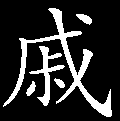
\includegraphics[width=3mm]{../Images/00005}总评:写贫贱辈低首豪门,凌辱不计,诚可悲乎!此故作者以警贫贱。而富室贵豪亦当于其间着意。}

{\href{../Text/part0044_split_000.html\#navto_1_a}{①}语出唐李商隐《宿骆氏亭寄怀崔雍崔衮》诗,原句作``留得枯荷听雨声''。}
